\documentclass{article}
\usepackage[utf8]{inputenc}
\usepackage{amsmath}
\usepackage{graphicx}
\usepackage{float}
\usepackage[hidelinks]{hyperref}

\title{Prática 1 - Aplicação Prática de conceitos sobre Cultura e Estrutura organizacional}
\author{Aluno: João Pedro Rodrigues Leite \\ RA: A2487055}
\date{}

\begin{document}
	
	\maketitle
	
	\subsection*{1) \textnormal{Pesquise um organograma de alguma empresa qualquer e cole-o na resposta. Utilizando este organograma, analise quais características de uma estruturas organizacionais se aplicam e a partir destas, explique e dê exemplo. Utilize por base as seguintes características:}}
	
	\begin{figure}[H]
		\centering
		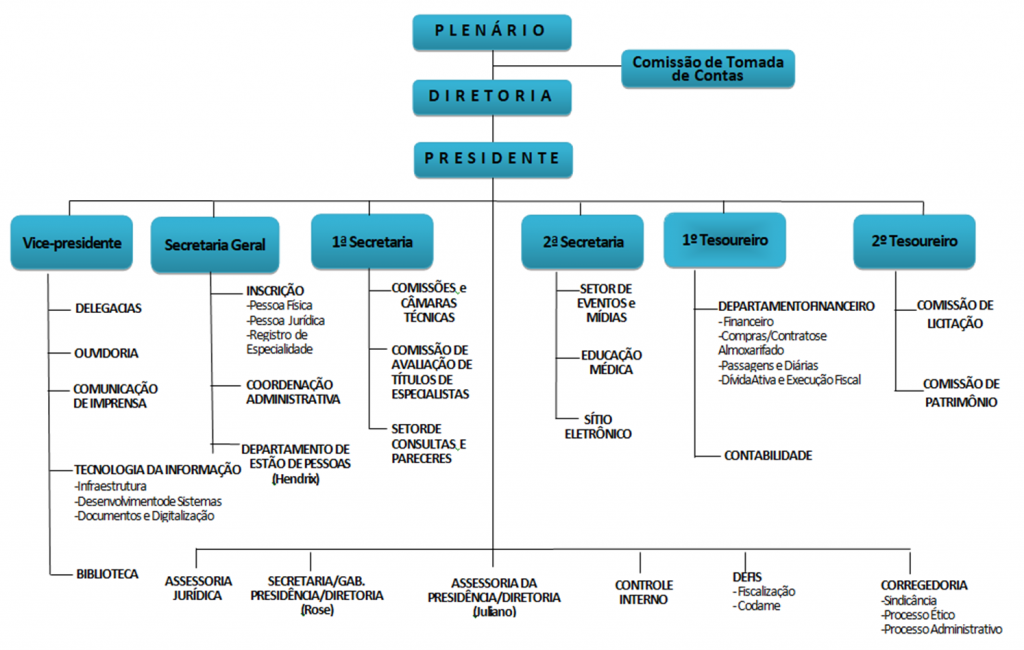
\includegraphics[width=1\linewidth]{figs/organograma-crmms}
	    \caption{Organograma da empresa CRM-MS. Fonte: \href{https://crmms.org.br/institucional-2/organograma}{CRM-MS}.}
		\label{fig:organograma-crmms}
	\end{figure}
		
	\subsubsection*{a) \textnormal{Hierarquia}}
	A hierarquia aqui é clara e organizada. O Plenário está no topo, seguido pela Diretoria, Presidente e as várias Secretarias e Tesouraria. Isso garante uma cadeia de comando bem definida e facilita a tomada de decisões.
	
	\subsubsection*{b) \textnormal{Amplitude de Controle}}
	O Presidente tem muitos subordinados diretos, como os Vice-Presidentes e Secretarias. Cada um desses líderes também supervisiona várias áreas, mostrando uma amplitude de controle ampla.
	
	\subsubsection*{c) \textnormal{Especialização}}
	A estrutura é bem especializada. Cada departamento tem funções claras, como a Tecnologia da Informação, que cuida de sistemas, enquanto o Departamento Financeiro foca em questões monetárias.
	
	\subsubsection*{d) \textnormal{Departamentalização}}
	A empresa está dividida em departamentos funcionais. Por exemplo, a Secretaria Geral cuida de TI e comunicação, enquanto a Tesouraria é responsável por finanças.
	
	\subsubsection*{e) \textnormal{Centralização/Descentralização}}
	Embora o Presidente tenha grande poder de decisão, os departamentos têm autonomia para gerenciar suas atividades, mostrando uma mistura de centralização e descentralização.
	
	\subsubsection*{f) \textnormal{Coordenação}}
	Os diferentes departamentos parecem trabalhar juntos para atingir os objetivos da organização. Por exemplo, o Departamento Financeiro precisa se coordenar com a Contabilidade também para manter em ordem a questão fiscal.
	
	\subsubsection*{g) \textnormal{Padronização}}
	As atividades parecem seguir processos padronizados, especialmente em áreas como o setor financeiro, onde a padronização é essencial para garantir a consistência.
		

	\subsection*{2) \textnormal{A partir das estruturas organizacionais funcional, projetizada e matricial, apresente organograma de 3 empresas(ou descrição textual)adequadas a cada estrutura. Justifique sua resposta}}

	\subsubsection*{a) Estrutura Funcional}
	- \textbf{Exemplo}: \textit{Unilever} \\
	- \textbf{Justificativa}: A Unilever usa uma estrutura funcional, dividindo a empresa em áreas especializadas, como marketing, vendas e produção. Isso significa que cada departamento foca em suas próprias tarefas e é especializado para fazer o que sabe. Assim, a Unilever consegue manter um padrão de qualidade e eficiência em seus produtos. \\
	- \textbf{Descrição do Organograma}: Na Unilever, o organograma é estruturado da seguinte forma: no topo, temos o Diretor Geral, que supervisiona todos os departamentos. Abaixo dele, existem gerentes funcionais responsáveis por áreas como Marketing, Vendas, Produção e Finanças. Cada gerente de departamento tem equipes específicas que lidam com tarefas diárias e relatórios regulares, garantindo que todos trabalhem de maneira alinhada com os objetivos da empresa.
	
	\subsubsection*{b) Estrutura Matricial Balanceada}
	- \textbf{Exemplo}: \textit{Apple} \\
	- \textbf{Justificativa}: A Apple trabalha com uma estrutura matricial balanceada, onde os gerentes de projeto e de departamento compartilham o poder. Isso ajuda a criar equipes que misturam talentos de diferentes áreas, como design e engenharia, para desenvolver os produtos. Dessa forma, eles conseguem garantir que tudo, desde a aparência até a funcionalidade, atenda às expectativas dos consumidores. \\
	- \textbf{Descrição do Organograma}: Na Apple, o organograma apresenta uma divisão onde o CEO está no topo, seguido por gerentes de departamentos funcionais, como Design, Engenharia, Marketing e Vendas. Além disso, há gerentes de projeto que lideram equipes formadas por membros de diferentes departamentos. Essas equipes são criadas especificamente para cada novo produto ou iniciativa, promovendo a colaboração e a comunicação entre áreas, resultando em inovações rápidas e eficazes.
	
	\subsubsection*{c) Estrutura Projetizada}
	- \textbf{Exemplo}: \textit{Google} \\
	- \textbf{Justificativa}: O Google adota uma estrutura projetizada, onde as equipes são montadas em torno de projetos específicos. Isso dá liberdade para os funcionários se concentrarem em suas ideias e inovações. Com esse modelo, eles conseguem ser ágeis e criativos, sempre prontos para lançar novos serviços e produtos que realmente fazem a diferença. \\
	- \textbf{Descrição do Organograma}: No Google o CEO está no topo, e logo abaixo existem gerentes de projeto que lideram equipes específicas. Cada equipe é composta por especialistas de várias áreas, como engenharia, marketing e design. Quando um projeto termina, a equipe pode ser reconfigurada para um novo projeto. Essa estrutura permite que os funcionários trabalhem de forma autônoma e criativa.
	
\end{document}
